\section{Statistics and inference}

\subsection{Basics of Statistics}
\subsubsection{Statistical Population}

Statistical population is the set of all possible elements that are of interest for a statistical analysis.
\begin{example}
    The time series of split-adjusted daily stock prices of Dell Inc. since IPO on June 22, 1988 till taken private on October 29, 2013.
\end{example}

\subsubsection{Moment Generating Function}
Let $X$ be a random variable with pdf $f(x)$. The moment generating function(mgf) of X is:
\[
    \begin{aligned}
        M_x(\theta) &= \mathbb{E}[e^{\theta x}]\\
        &= 1 + \mathbb{E}[x]\theta + \mathbb{E}[x^2]\frac{\theta^2}{2!} + \mathbb{E}[x^3]\frac{\theta^3}{3!} + \cdots
    \end{aligned}
\]

$M_x^n(0)$ gives us the $n$th moment of the distribution of the random variable $x$:
\begin{itemize}
    \item $\mu = M_x^1(0)$ 
    \item $\sigma^2 = \mathbb{E}[x^2]-(\mathbb{E}[x])^2 = M_x^2(0) - (M_x^1(0))^2$
    \item $\mathrm{Skewness} =  \mathbb{E}(x^3) - 3 \mathbb{E}(x) \mathbb{E}(x^2) +2 (\mathbb{E}(x))^3$\\
    \phantom{}\qquad \qquad \,$=   M_x^3(0) - 3(M_x^1(0))^2M_x^2(0) + 2(M_x^1(0))^3   $
    \item $\mathrm{Kurtosis} = \mathbb{E}(x^4) - 4\mathbb{E}(x)\mathbb{E}(x^3) + 6(\mathbb{E}(x))^2\mathbb{E}(x^2) - 3(\mathbb{E}(x))^4$
\end{itemize}
\begin{remark}
    Because typing seperated equations under environment "itemize" will cause some problems, so I just typed skewness as an example of subsitute moment of x with mgf.
\end{remark}

\subsubsection{Linear Combination of Variables: Mean and Variance}
Let $a$,$b$ and $c$ be constant. Let $X$ and $Y$ be two random variables, with means $\mu_X$ and $\mu_Y$ respectively. Also, the corresponding variances are $\sigma_X^2$, $\sigma_Y^2$, Then

\begin{itemize}
    \item $\mathbb{E}(aX+bY+c) = a\mathbb{E}(x) + b\mathbb{E}(Y) + c$
    \item $\mathbb{V}(aX+bY+c) = a^2\mathbb{V}(X) + b^2\mathbb{V}(Y) +2ab\mathbb{C}(X,Y)$
\end{itemize}

Where $\mathbb{C}(X,Y) = \mathbb{E}(XY) - \mathbb{E}(X)\mathbb{E}(X)$.

\subsubsection{Population versus Sample}
Population parameters (e.g. mean, variance, etc) are usually unobserved. But if we assume that the dataset follows a certain parametric distribution (say “normal”), then we can try to estimate the parameters of that distribution from the data.

Properties of estimators:
\begin{itemize}
    \item \textbf{Bias}: Bias is the difference between the expected value of the estimator and the true (unobserved) parameter value being estimated. A zero bias estimator is an unbiased estimator.
    \item \textbf{Consistency}: Estimators are typically computed over a finite sample size n. Consistency refers to how, as n increases, the estimated value gets closer and closer to the true parameter value.
    \item \textbf{Efficiency}: For an unbiased estimator, efficiency refers to how much its precision is lower than the theoretically highest possible precision. A more efficient estimator needs fewer observations to achieve a given level of variance (precision).
\end{itemize}

\textbf{Unbiasedness}

A statistic $\Psi(X)$is an unbiased estimator of $\theta$ if
\[
    \mathbb{E}[\Psi(X)] = \theta
\]

For population's observations $R_1,R_2,\cdots,R_n$, we have \textbf{unbiased estimate of mean and variance} for population as follows:
\[
    \begin{aligned}
        \mu &= \frac{1}{n}\sum_{t=1}^{n}R_t\\
        \sigma^2 &= \frac{1}{n-1}\sum_{t=1}^{n}(R_t-\mu)^2
    \end{aligned}
\]

\textbf{Consistency}

A sequence of estimators $\theta_n(X)$ of $\theta$ from sample $X$ of size $n$ is said to be a consistent estimator if
\[
    \lim_{x \to +\infty}\mathbb{P}(\theta_n - \theta |<\epsilon) = 1
\]



\subsection{Statistical Distribution}
The statistical Distribution of a variable’s population is a description of the relative numbers of times each possible outcome will occur in a number of trials.

\subsubsection{Normal Distribution}
If $X \stackrel{d}{\sim} \mathcal{N}(\mu,\sigma^2)$, the PDF $f(x)$ is 
\[
f(x) = \frac{1}{\sqrt{2\pi \sigma^2}} \exp(-\frac{1}{2}(\frac{x-\mu}{\sigma})^2)
\]

Mean and Variance:
\[
\begin{aligned}
    \mathbb{E}(x) &= \int_{-\infty}^{\infty}xf(x)dx = \mu\\
    \mathbb{V}(x) &= \int_{-\infty}^{\infty}(x-\mu)^2 f(x)dx = \sigma^2
\end{aligned}    
\]

Let $\mu = 0, \sigma^2 = 1$, we have pdf:
\[
f(x) = \frac{1}{\sqrt{2\pi}}\exp(-\frac{x^2}{2})    
\]

\subsection{Statistical Inference}
\subsubsection{Law of Large Number(LLN)}
\begin{theorem}{Law of Large Number(LLN)}
    For random sample $X_1,X_2,\cdots,X_n$, if $n$ is large enough, the expectation of variance $X$ equals to mean of samples:
    \[
    \mathbb{E}[X] = \lim_{n\to \infty}\frac{1}{n}\sum_{t=1}^{n}X_t
    \]
\end{theorem}

\subsubsection{Central Limit Theorem(CLT)}
\begin{theorem}{Central Limit Theorem(CLT)}
    Suppose ${X_1,X_2,\cdots,X_n}$ is a sequence of \textbf{independent and identically distributed}(i.i.d.) random variables with $\mathbb{E}[X_t] = \mu$ and variance $\mathrm{Var} = \sigma^2 < \infty$. As $n$ approches infinity, the distribution of sum $X_t$ converges to a  normal distribution:

    \[
        \sum_{t=1}^nX_t \sim \mathcal{N}(n\mu,n\sigma^2)
    \]
\end{theorem}

\subsubsection{Confidence Interval}
Suppose data ${X_1,X_2,\cdots,X_n}$ are randomly sampled from $X \sim \mathcal{N}(\mu,\sigma^2)$ such that for an $a > 0$:
\[
    \mathbb{P}(-a<t<+a) = 95\%
\]
Where $\frac{\sqrt{n}(\overline{X}-\mu)}{\sigma}=t\sim \mathcal{N}(0,1)$(CLT), so we know the value of $a$.

Thus the probability of $\mu$ falling within the confidence interval $[\overline{X}-a\frac{\sigma}{\sqrt{n}}, \overline{X}+a\frac{\sigma}{\sqrt{n}}]$ is 95\%:

\[
    \mathbb{P}(\overline{X}-a\frac{\sigma}{\sqrt{n}}\leq \mu \leq \overline{X}+a\frac{\sigma}{\sqrt{n}}) = 95\%
\]

This probability of 5\% is known as the \textbf{significance level}. The \textbf{critical regions} correspond to the significance level's areas.

\subsubsection{Type I and Type II Errors}

\begin{figure}[!ht]
	\centering
	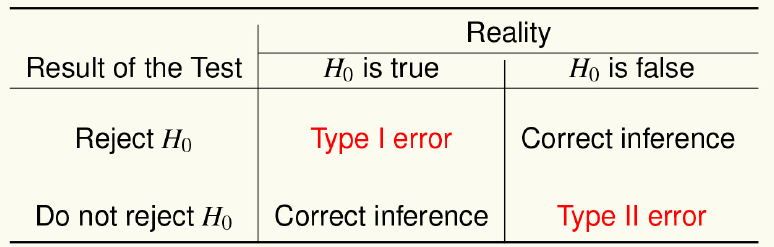
\includegraphics[width=\textwidth]{typeI_II_errors.png}
	\caption{Type I and Type II Errors}
\end{figure}
